\documentclass{../src/bcthesispart}
\title{Bayesian Language Games}
\author{Bas Cornelissen}
\begin{document}


%——————————————————————————————————————————————————————————
\parttitle{Bayesian Language Games}%
	{Bayesian Language Games}%
	{bayesian-naming-games}%
	{% Abstract
	Few studies, it seems, have tried to bridge the gap between iterated learning and naming games.
	In this chapter I argue that Bayesian models of iterated learning can naturally be connected to naming games in the form of a new, Bayesian language game.
	This model of cultural evolution gives rise to a stable, lineage-specific language that reflects innate biases, but not faithfully so.
	With a proposed population structure, the game interpolates between an iterated learning model and a naming game and moreover incorporates a wide range of strategies.
	The model, in short, brings a unified perspective on two agent-based modelling paradigms and addresses some of the desiderata formulated in chapter \ref{ch:iterated-learning}.
	}
%——————————————————————————————————————————————————————————




\noindent
Naming games and iterated learning are the central traditions of agent-based modelling of language evolution \parencite{Smith2014,Grifoni2016,Jaeger2009}.
In \textcite{Jaeger2009} they even form the axes defining the space of agent-based simulations: naming games horizontally and iterated learning vertically.
But the coordinate system looks rather empty.
Although horizontal and vertical models have often been combined, the interaction between the two traditions seems extremely limited.
A naive citation count makes this disturbingly clear.\footnote{%
	%>>> 
	I counted references to papers coming from the group of either Kirby (\textsc{il}) or Steels (\textsc{ng}). 
	All serious papers in either tradition cite extensively from the work of the respective groups.
	%<<<
}
A paper by Luc Steels (2016) \nocite{Steels2016} with the inclusive title \emph{Agent-based models for the emergence and evolution of languages} cites a grand total of zero iterated learning papers.
Some years earlier, \textcite{Steels2011} scores 3/120 in a review called \emph{Modelling the cultural evolution of language}.
At least the traditions meet in mutual neglect:
\emph{The cultural evolution of language} \parencite{Tamariz2016} scores\footnote{%
	%>>>
	Admittedly, \textcite{Tamariz2016} \emph{does} cite the experimental semiotics literature. But then again, it does \emph{not} include Steels under the heading ‘naming games’ (table 1), under which we do find some papers from Kirby’s group.
	%<<<
	}
1/73 and \textcite{Kirby2014} 2/60. 
But then again, the latter paper is called \emph{Iterated learning and the evolution of language}.
%%
 
 
 
 

A case of incommensurable paradigms?
In this chapter, I will argue the opposite.
Far from being incommensurable, Bayesian models of iterated learning and naming games naturally meet in a model I will call the \emph{Bayesian language game}.
This will be the extension of a Bayesian \emph{naming} game, to be introduced first.
Several closely related models can be found in the literature, but, to the best of my knowledge, have never been used to connect the two traditions.
I review related work at the end of this chapter and would like to start where we left off in the previous chapter: the convergence proof of the naming game.
%%




%——————————————————————————————————————————————————————————
%——————————————————————————————————————————————————————————
\section{The Bayesian naming game}
%——————————————————————————————————————————————————————————
%——————————————————————————————————————————————————————————


The \emph{Bayesian naming game} can be seen as an extension of the naming game studied by \textcite{DeVylder2006}.
We make similar simplifications and assume all $N$ agents already know words $w_1, \dots, w_K$, and need to negotiate which of these words to use for the single object at hand.
Each agent has an internal language $\vlang$, a distribution over the $K$ words, based on which it produces words $\vobs$ using some production strategy.
I use this naming game interpretation throughout the chapter, but it should be noted that the language $\vect\theta$ has also be interpreted as a distribution over various linguistic variants.
As \textcite{Reali2010} explain, “learning a language involves keeping track of the frequencies of variants of a linguistic form at various levels of representation, including phonology, morphology, and syntax”.
\textcite{Ferdinand2009} represent languages in a similar fashion.



The queue-learners in \textcite{DeVylder2006} ‘learned’ their language by computing the relative frequencies of observed words.
Here, the Bayesian naming game takes a different turn.
Following Bayesian iterated learning models, it assumes that agents are Bayesian reasoners updating their language using Bayes’ rule.
In other words, they use Bayesian updating as an \emph{alignment strategy}.
After observing utterances $\vobs$, the agent infers the posterior distribution over languages
%-
\begin{align}
	\label{eq:ch4:bayesian-inference}
	%-----
	p(\vlang \mid \vobs) 
		\propto 
			p(\vobs \mid \vect \vlang) 
			\cdot p(\vlang),
\end{align}
%-
and \emph{samples} a language accordingly (other strategies are discussed later).
Just like iterated learning models, the biases of the agent enter the model explicitly in the form of a prior $p(\vlang)$. 
But there is an important difference.
Agents engage in multiple encounters and every time a hearer interact, its \emph{beliefs} about the language it should use, have to be updated.
The the posterior beliefs $p(\vlang \mid \vobs_t)$ inferred during interaction $t$ should thus serve as the prior beliefs $p_{t+1}(\vlang)$ in round $t+1$.
Strictly speaking, I use ‘prior’ as a technical term for the distribution $p_t(\vect\theta)$.
It can be \emph{interpreted} as the ‘beliefs’ of the agent.
In the first round, the prior encodes the \emph{(innate) biases}, but later in the game, it encodes both innate biases and \emph{past experience}.
For simplicity, I consistently speak of \emph{innate} biases, but a more more precise reading would be “everything that the learner brings to the task independent of the data” \parencite{Kirby2004}. The distinction becomes relevant in chapter \ref{ch:counting-games}.
%%




In general terms, round $t$ in the Bayesian naming game has the following script.
%...
\begin{itemize}
	\item A hearer $H$ and speaker $S$ are randomly selected from the population.	

	\item The speaker samples a language $\vlang_t$ from her prior distribution $p_{S,t}(\vlang)$. This is the posterior $p_{S}(\vlang \mid \vobs_{t'})$ inferred during the last interaction $t'$ she engaged in as a hearer. The selected language defines a distribution $p(x \mid \vlang_t)$ over words. She samples $b$ words $\vobs_t = (\obs_1, \dots, \obs_b)$ from that distribution and communicates those to the hearer.

	\item The hearer updates his beliefs $p_{H, t+1}(\vlang) := p_H(\vlang \mid \vobs_t)$ to the posterior, which is proportional to $p(\vobs_t \mid \vlang)\cdot p_{H, t}(\vlang)$. 
		All other agents $A$, including the speaker, maintain their current beliefs: $p_{A,t+1}(\vlang) := p_{A, t}(\vlang)$.
\end{itemize}
%...
This script outlines a general framework for Bayesian naming games.
This chapter discusses one specific instantiation, a \emph{Dirichlet-categorical naming game}, but it should be noted that the proposed framework is more general.
%%



On a practical note, a mathematical development of the model is included in appendix \ref{app:bng}.
The treatment in the main text is informal and to keep the notation uncluttered, deliberately sloppy:
I do not decorate variables with the corresponding agent, time or index, unless strictly necessary.
%%




%- - - - - - - 
\begin{SCfigure}
	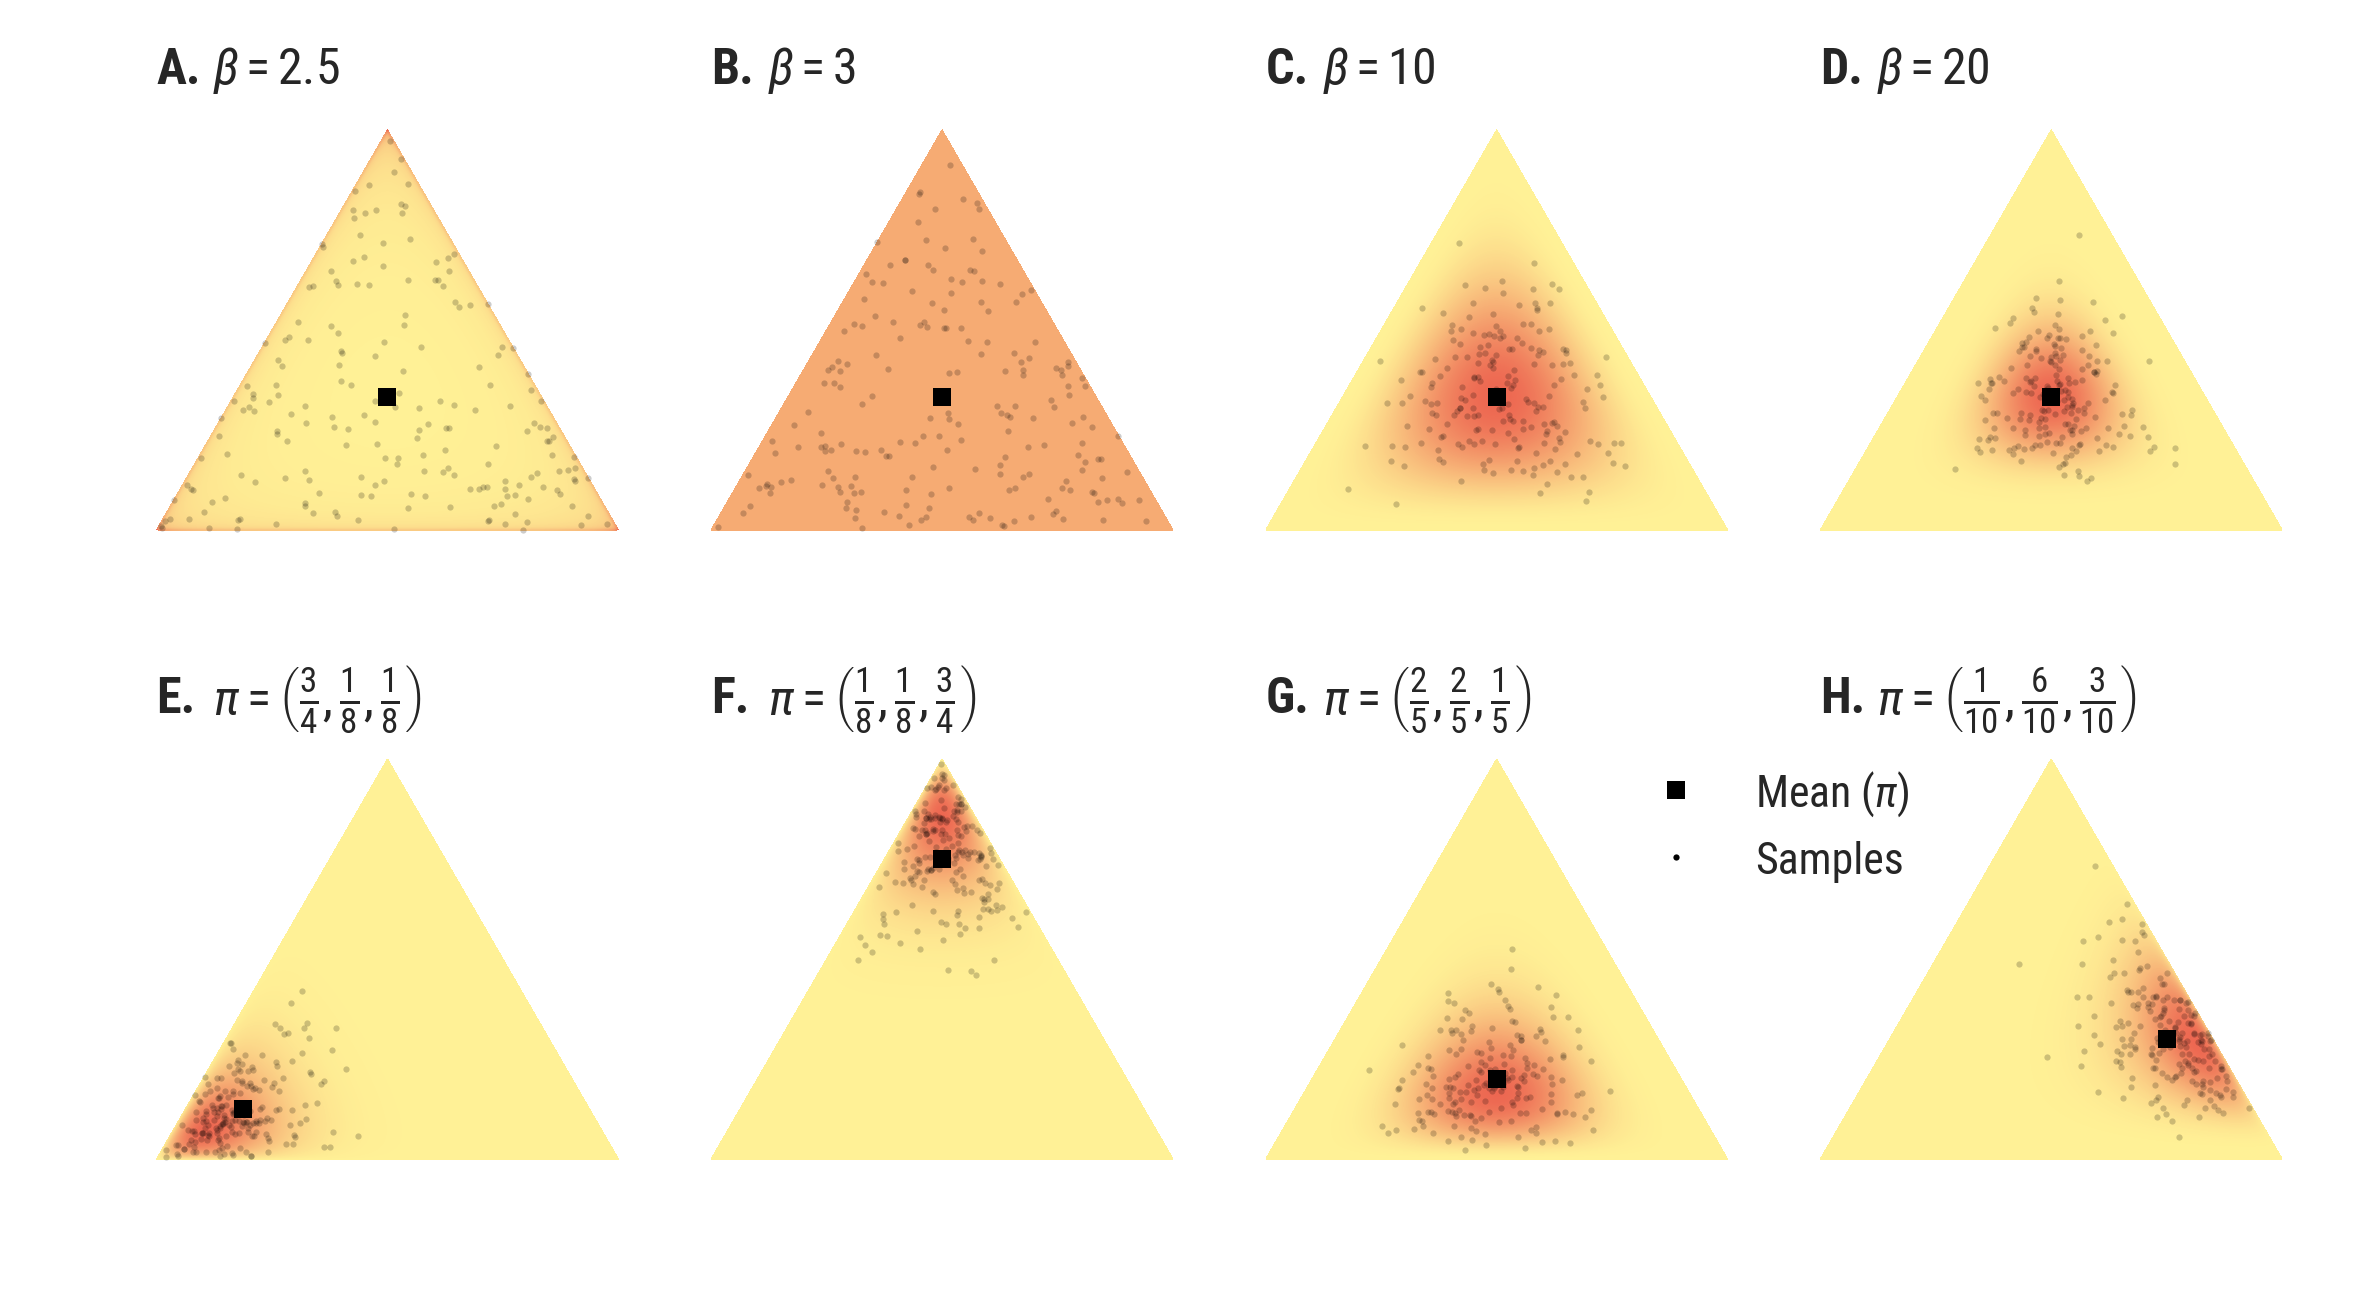
\includegraphics[trim=0.94cm 0 0 \figtopmargin]{FIG02-dirichlet-parameters}
	
	\caption{
	The Dirichlet distribution for various parameter settings. 
	The Dirichlet can be parametrised by a point $\vect\mu$ in the simplex and a scalar $\beta$. 
	The mean of the distribution is determined by $\vect\mu$ and $\beta$ influences the variance.
	The first row (A--D) demonstrates the effect of $\beta$ while fixing $\vect\mu=(\nicefrac13, \nicefrac13,\nicefrac13)$; 
	the second row (E--H) the effect of $\vect\mu$ while keeping $\beta=15$ fixed. 
	Note that with $\beta\cdot\vect\mu = (1,1,1)$ (subfigure B) one gets a uniform distribution over the simplex.
	%----------
	\figdetails{\figid{fig02} %
	Figure produced using code by Thomas Boggs at \href{https://gist.github.com/tboggs/8778945}{gist.github.com/tboggs/8778945}}
	\label{fig:dirichlet-parameterisation}}
\end{SCfigure}
%- - - - - - -



%——————————————————————————————————————————————————————————
\section{The Dirichlet-categorical naming game}

Following \textcite{DeVylder2006}, the internal language $\vlang$ of an agent is a categorical distributions over words, but what should the prior distribution over languages look like?
The obvious candidate is the \emph{Dirichlet distribution}, because it is the \emph{conjugate prior} of the categorical.
This means that the posterior distribution has the same parametric form as the prior, i.e.~the posterior will also be a Dirichlet.
If the prior at time $t$ is parametrised by some parameter vector $\vect\alpha_t$, the \emph{hyperparameter}, then posterior inference amounts to determining the new hyperparameter $\vect\alpha_{t+1}$, which can often be done analytically.
So in terms of the Bayesian naming game, hearers only need to change the hyperparameter after an interaction to update their beliefs.




The Dirichlet distribution is defined over the \emph{entire} simplex — not just over the finite subset $\simplex_Q$, as with the multinomial in \textcite{DeVylder2006} — and thus assigns a probability to \emph{every} language, \emph{every} distribution over $K$ words.
It is parametrised by a vector $\vect \alpha = (\alpha_1, \dots, \alpha_K)$, but it is often convenient to split this into a normalised vector $\mathbf\mu$ and a scalar parameter $\beta>0$ and use $\vect\alpha = \beta\cdot\vect\mu$.
The vector $\vect\mu$, since it sums to 1, lies in the simplex and determines the mean of the distribution.
$\beta$ is a kind of inverse variance, with larger values of $\beta$ resulting in smaller variance.
Figure \ref{fig:dirichlet-parameterisation} illustrates different parameterisations oft 




With this conjugate prior, posterior inference amounts to updating the hyperparameter $\vect\alpha$ — but how?
Suppose the hearer receives words $\vobs_t = (\obs_1, \dots, \obs_b)$ — here $b$ is the \emph{bottleneck size} — and let $\vect c_t = (c_1, \dots, c_K)$ denote the corresponding vector of counts, such that $c_k$ is the number of $k$’s in $\vobs$.
If $\vect\alpha_t$ is the previous hyperparameter, then the posterior of the hearer is
%-
\begin{align}
	p(\vlang \mid \vobs_t) = 
		\text{Dirichlet}(\vlang \mid \vect\alpha_t	+ \vect c_t),
\end{align}
%-
and the belief update amounts nothing more than $\vect\alpha_{t+1} := \vect\alpha_t + \vect c_t$.
The \emph{Dirichlet-categorical} (\textsc{dc}) naming game we have defined can now be summarised as 
%-
\begin{align}
	\textsc{speaker}
	\quad
	&\begin{cases}
		\vlang_t \mid \vect\alpha_{t-1}
			&\sim \text{Dirichlet}\bigl(\vect\alpha_{t-1}\bigr)\\
		x_i \mid \vlang_t
			&\sim \text{Categorical}\bigl(\vlang_t\bigr), \quad i = 1, \dots, b.
	\end{cases}
	\\
	\textsc{hearer}
	\quad
	&\;\;\vect\alpha_{t+1} 
		:= \vect\alpha_{t} + \vect c_t
\end{align}
%-
Note that the speaker still \emph{samples} both languages and productions.
Other strategies are discussed later.
%%




%- - - - - - - - 
\begin{SCfigure}
	\hspace{-.9cm}
	%\documentclass{../src/bcthesispart}
%\begin{document}
\begin{tikzpicture}[xscale=2.4]\footnotesize\sffamily
	\tikzset{var/.style={draw, circle, fill=main!60, minimum size=.75cm}}
	\tikzset{sample/.style={thick, draw, ->}}
	\tikzset{ann1/.style={align=center, text width=2cm, node distance=2.5cm, text=main}}
	\tikzset{ann2/.style={align=center, text width=2cm, node distance=1.3cm,text=main}}
	\tikzset{annline/.style={draw,dashed,main}}
	\tikzset{speaker/.style={draw}}
	\tikzset{hearer/.style={draw}}
	\tikzset{brace/.style={decoration={brace,mirror,raise=10pt}, decorate}}

	\draw[speaker] (-.95,0) rectangle (2,1.75);
	\node[] at (-.7, .25) {\textsc{speaker}};
	
	\node[var] (alpha) at (0,1) {$\vect\alpha_t$};
	\node[left of=alpha,align=right] (observations) {$\vect c_{-t}$};
	\node[left of=observations,align=right] (bias) {$\vect\alpha_0$};
	\path (observations) -- node {$=$} (alpha);
	\path (bias) -- node{$+$} (observations);
	\node[var] (lang) at (1,1) {$\vlang_t$};
	\node[var] (obs) at (2.35,1) {$\obs_t$};
	
	\draw[sample] (alpha) -- 
		node[above] (langdist) {$p_\LA(\vlang_t \mid \vect\alpha_t)$}
		(lang);
	\draw[sample] (lang) -- 
		node[above,pos=.44] (proddist) {$p_\PA(x_t \mid \vlang_t)$}
		(obs);
	\draw[sample] (alpha) to[out=-60,in=-120,max distance=.75cm]
		node[above,pos=.54] (pi) {$\vect\pi_t$}
		(obs);
	
	\node[ann1,above of=lang] (a1) {\emph{internal}\\ language};
	\draw[annline] (a1) -- (lang);
	\node[ann2,above of=obs, node distance=1.45cm] (a2) {production};
	\draw[annline] (a2) -- (obs);
	\node[ann1,above of=alpha] (a3) {beliefs};
	\draw[annline] (a3) -- (alpha);

	\node[ann2,above of=langdist] (a4) {language\\ algorithm};
	\draw[annline] (a4) -- (langdist);
	\node[ann2,above of=proddist, node distance=2.27cm] (a5) {production\\ algorithm};
	\draw[annline] (a5) -- (proddist);
	\node[ann1,above of=pi, node distance=2.1cm] (a6) {\emph{average}\\language};
	\draw[annline] (a6) -- (pi);
	
	\node[ann1,above of=bias] (a7) {innate\\bias};
	\draw[annline] (a7) -- (bias);
	\node[ann2,above of=observations, node distance=1.4cm] (a8) {observations\\or experience};
	\draw[annline] (a8) -- (observations);
	
	\draw[hearer] (2.7,0) rectangle (4.1,1.75);
	\node[] at (2.95, .25) {\textsc{hearer}};
	\draw[thick,->] (obs) -- (2.7, 1);
	
	\node[align=left] at (3.35, .7) {$\vect\alpha_{t+1} := \vect\alpha_t + \vect c_t$};
	
	\node (posterior) at (3, 1.2) {$p_{t+1}(\vlang)$};
	\node[right of=posterior, node distance=1.3cm] (likelihood) {$p(x_t \mid \vlang)$};
	\node[right of=likelihood] (prior) {$p_t(\vlang)$};
	\path (posterior) -- node {$\propto$} (likelihood);

	\node[ann1,above of=posterior, node distance=2.25cm] (a9) {posterior\\(next prior)};
	\draw[annline] (a9) -- (posterior);

	\node[ann2,above of=likelihood, node distance=1.25cm] (a10) {likelihood};
	\draw[annline] (a10) -- (likelihood);
	
	\node[ann1,above of=prior, node distance=2.15cm] (a11) {prior};
	\draw[annline] (a11) -- (prior);

	\newcommand{\drawinteraction}[2]{
		\def\y{#1}
		\def\t{#2}
		\begin{scope}[yshift=\y]
			\draw[speaker] (-.95,0) rectangle (2,.5);
			\node[] at (-.7, .25) {\textsc{speaker}};
			
			\node[var] (obs) at (2.35,.25) {$\obs_{t+\t}$};
			\draw[sample] (2, .25) -- (obs);
			\draw[thick,->] (obs) -- (2.7, .25);
			
			\draw[hearer] (2.7,0) rectangle (4.1,.5);
			\node[] at (2.95, .25) {\textsc{hearer}};
		\end{scope}
	}
	
	\drawinteraction{-1cm}{1}
	\drawinteraction{-2cm}{2}
	
	\draw[dotted,thick] (2.08,2) -- (2.08,-2.3) -- (2.62, -2.3) -- (2.62,2);

	\draw [brace] (2.08, -2.1) -- (2.62,-2.1) 
    	node [pos=0.5, yshift=-.7cm, text width=4cm, align=center] (psi) {$\vect\psi_{t+2}$};
    \node[below of=psi,text=main, node distance=.4cm] {\emph{external} language};
    	
\end{tikzpicture}
%\end{document}

	
	\caption{%
	Illustration of the Bayesian naming game with all relevant concepts. See main text for details.
	\label{fig:ch4-bng-terminology}}
\end{SCfigure}
%- - - - - - - - 




%——————————————————————————————————————————————————————————
\paragraph{Priors, beliefs, innate biases, and past experience}

An additional benefit of the \DC{} naming game is that it transparently represents several important concepts, which is visualized in figure \ref{fig:ch4-bng-terminology}.
First of all, we can separate beliefs from the prior. 
I will call the hyperparameter $\vect\alpha_t$ the \emph{beliefs}, since those are updated after every interaction, and the distribution $\text{Dirichlet}(\vect\alpha_t)$ the \emph{prior}.
Recall that the prior at $t=0$ encodes the innate biases, but in later encounters captures past experience as well.
Unraveling successive updates of the beliefs brings this fact to the fore:
%-
\begin{equation}
	\label{eq:ch4:unraveled-updates}
	%-----
	\vect\alpha_{t+1} 
		\;=\; \vect \alpha_0 + \vect c_1 + \vect c_2 + \dots + \vect c_t 
		\;=\; \vect\alpha_0 + \vect c_{-t},
\end{equation}
%-
where $\vect c_{-t}$ is the vector of counts of all observations before and including round $t$.\footnote{%
	%>>>
		We set $\vect c_t = 0$ if the hearer did not participate in round $t$.
	%<<<
	}
That is, $\vect c_{-t}$ captures all \emph{past experience}, whereas $\vect\alpha _0$ captures “everything that the learner brings to the task independent of the data” \parencite{Kirby2004}.
Equation \ref{eq:ch4:unraveled-updates} thus makes explicit that the beliefs in round $t$ are the sum of innate biases $\vect\alpha_0$ and past experience $\vect c_{-t}$.
It also shows that the innate biases act as so called \emph{pseudo-counts} of \emph{pseudo-observations}.
It is as if a newborn agent has already observed utterances with word counts given by $\vect\alpha_0$, before engaging in any interactions.
The point of \textcite{Griffiths2007a}, that the \emph{prior} should not be seen as the innate bias, is even more to the point here.
Alternatively, it can indeed be seen to regulate the amount of evidence needed to adopt a certain language.
If $\vect\alpha_t$ for example contains nothing but 20 observations of word $w_3$, the agent will need a lot of evidence before it will prefer to choose another word — irrespective of whether it concerns \emph{pseudo} or \emph{actual} observations.
%%




%——————————————————————————————————————————————————————————
\paragraph{Internal, external, expected and aggregate languages}

\emph{Languages}, here, are always distributions over words $w_1, \dots, w_K$, but care should be taken to distinguish several different distributions.
First of all, in every round the speaker chooses a language $\vlang_t$ from which she generates words.
This is the \emph{internal} language (\textsc{i}-language).
It is distinct from the \emph{external} language (\textsc{e}-language) which consists of all utterances.
The external language can be estimated with the relative frequencies of the words
%-
\begin{equation}
	\vect\psi_t := \frac{1}{b\cdot t}\cdot\sum_{\tau=1}^t c_\tau
\end{equation}
%-
In that way the external language $\vect\psi_t$ also becomes a distribution over words.




Finally, we need to introduce the \emph{expected} language and the \emph{aggregate} language for practical reasons.
Every agent entertains a full distribution over internal languages (the Dirichlet) and we cannot know beforehand which language it will use in a particular round. 
To probe the internal state of an agent we turn to its \emph{expected language} $\vect \pi_t = (\pi_1, \dots, \pi_K)$, the language it is expected to use in the next round. 
That is, we consider the marginal distribution
%-
\begin{align}
	\pi_k 
		&:= \; p\bigr(x = w_k \mid \vect\alpha_{t-1}\bigl)
		=\; \int_{\simplex} 
			p(x, \vlang \mid \alpha_{t-1}) 
			\; d\vlang
		\;=\; \hat{\alpha}_k,
\end{align}
%-
where $\hat{\alpha}_k$ is the $k$’th entry of $\hat{\vect\alpha}_t= \vect\alpha_t/\sum_j \alpha^{(t)}_j $, which is the normalised version of $\vect\alpha_t$.
The conjugacy of the Dirichlet gives this marginal distribution a simple form: the expected language $\vect\pi_t$ is proportional to the beliefs $\vect\alpha_t$ of the agent. 
Note that the expected language at $t=0$ is the language completely determined by the innate biases: $\vect\pi_0 = \hat{\vect\alpha}_0$. 
Accordingly, we often identify the bias with $\hat{\vect\alpha}_0$.
Finally, the average of the expected languages of all agents in the population is called the \emph{aggregate language}
%-
\begin{align}
	\bar{\vect\pi}_t 
		:= \frac{1}{N} \sum_{i=1}^N \vect\pi_{A_i,t},
\end{align}
%-
consistent with our terminology in chapter \ref{ch:naming-games}.
%%




%——————————————————————————————————————————————————————————
%——————————————————————————————————————————————————————————
\section{Phenomenology of the \textsc{dc} naming game}
%——————————————————————————————————————————————————————————
%——————————————————————————————————————————————————————————




%- - - - - - - - 
\begin{SCfigure}
	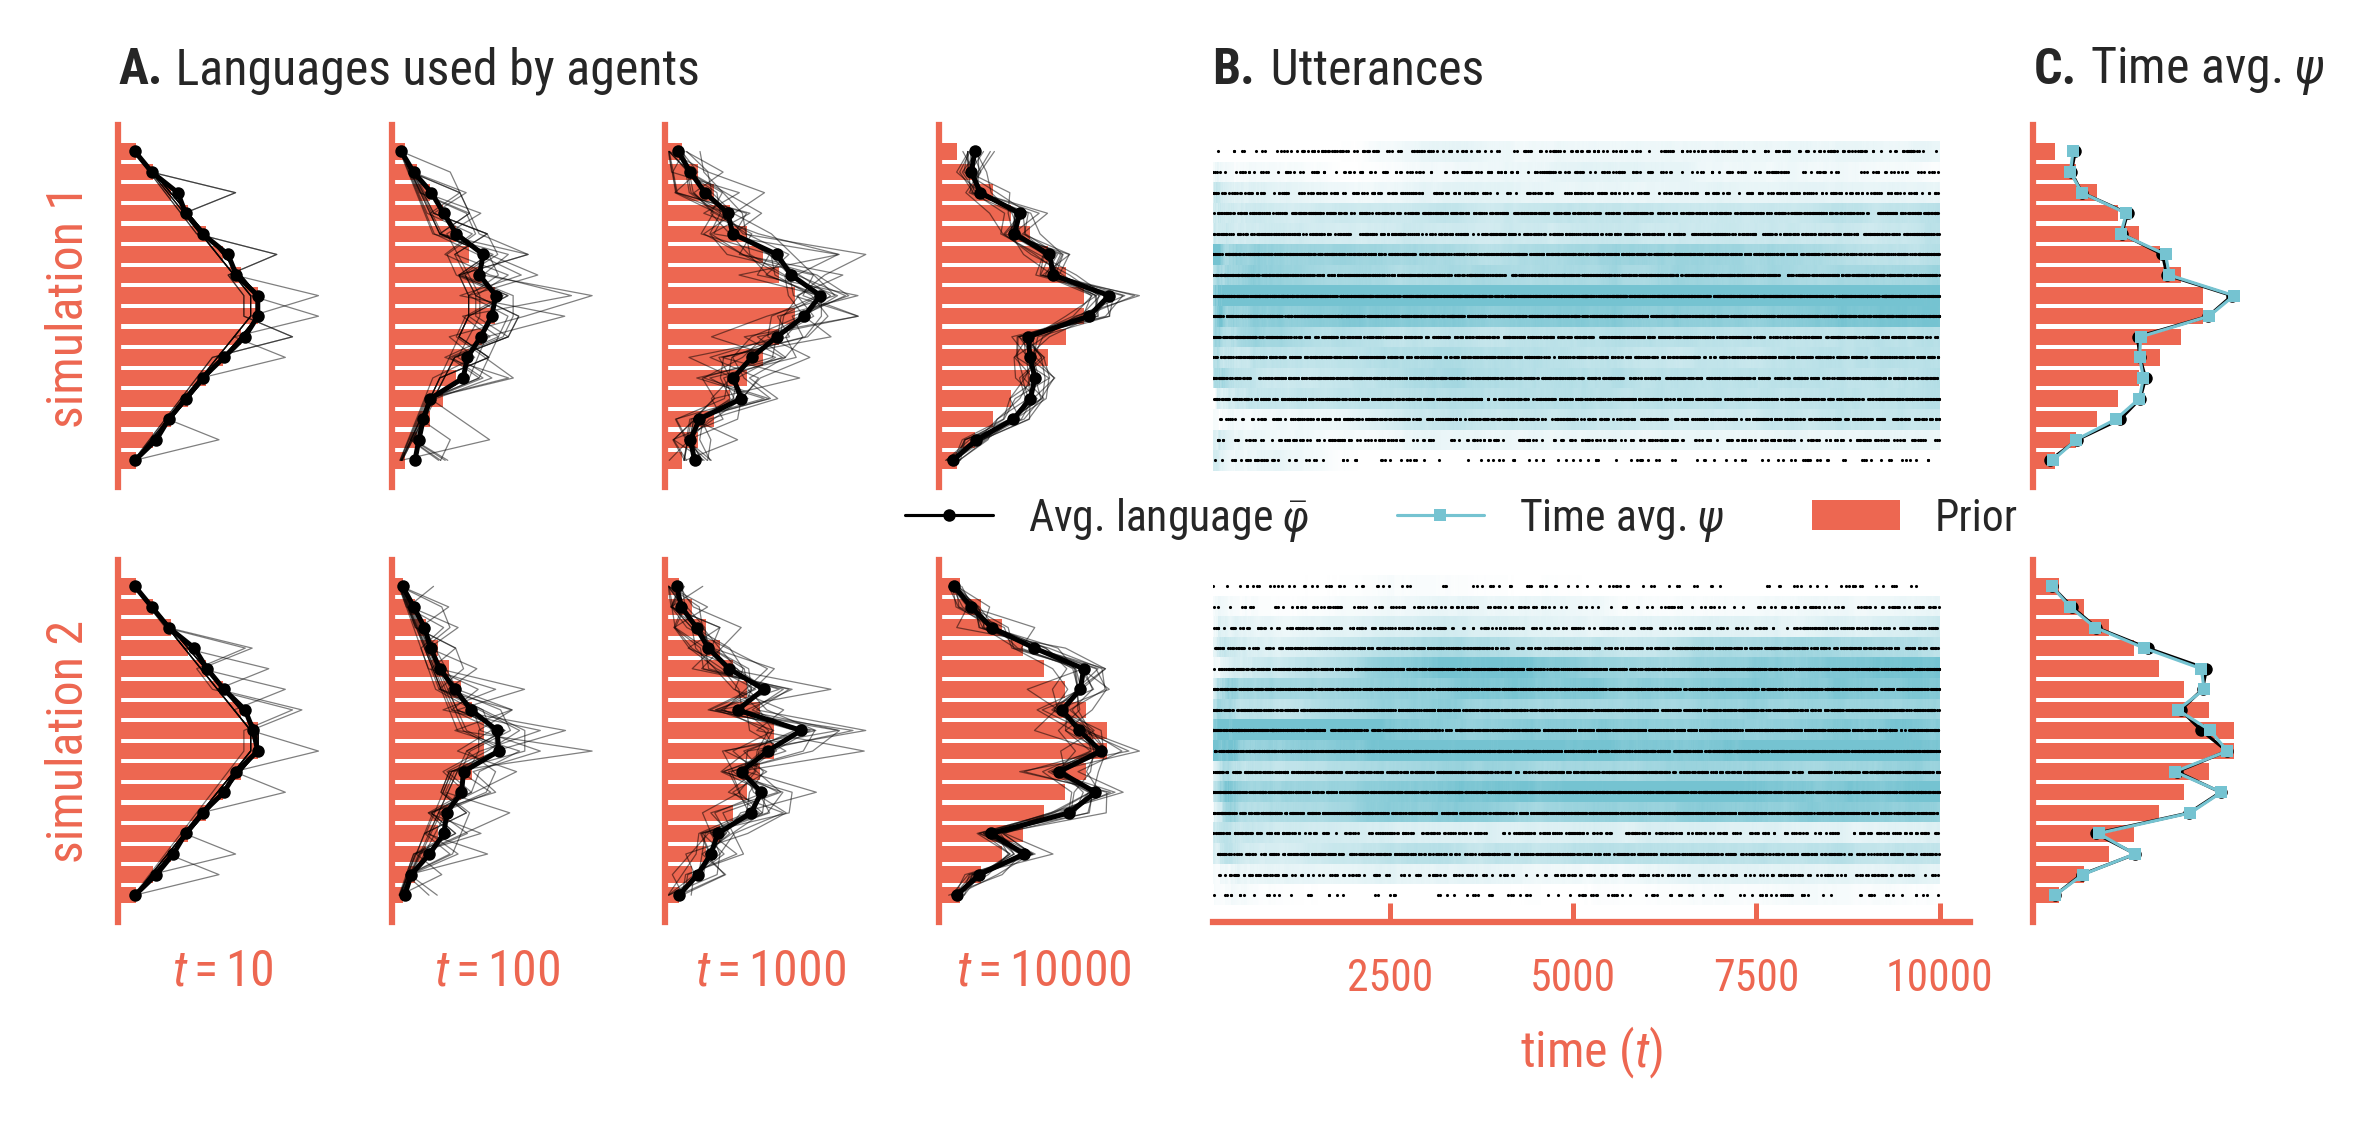
\includegraphics[trim=0.64cm 0 0 \figtopmargin]{FIG05-BNG-gamma-inf-zeta-1-eta-1-legend}
	\caption{Two runs of the Bayesian Naming Game. 
	\subfig{A} The distributions of all agents (thin black lines) first diverge but eventually stabilise. They always reflect the prior (orange),
	\subfig{B} Utterances (dots) at every time plotted over a moving average of 2000 time steps. 
	\subfig{C} The relative frequency of all utterances reflects the language  adopted in the population.
	See main text for more details.
		\figdetails{\figid{fig05} $K=16$, $N=15$, $b=1$, $\beta=18$, $\eta=\zeta=1$, $\gamma=\infty$}
		\label{fig:FIG05}}
\end{SCfigure}
%- - - - - - - - 





%——————————————————————————————————————————————————————————
\paragraph{three-stage evolution}

Figure \ref{fig:FIG05} show two typical runs of the Dirichlet-categorical naming game.
Subfigure \textsc{a} shows the expected languages of all the agents ($\vect\pi_A$, thin lines) and the aggregate language ($\bar{\vect\pi}$, thick lines) after 10, 100, 1000 and 10000 encounters. 
The cultural evolution can be divided in three stages, which I will metaphorically call ‘infancy’, ‘puberty’ and ‘adulthood’.
In ‘infancy’, the agents have engaged in few encounters and the innate biases ($\vect\alpha_0$, orange) have a strong effect on the language they use.
These ‘infants’ are fast learners: a single observation can drastically alter their beliefs.
But they have not yet accumulated enough evidence to develop a consistent, more or less stable language.
After a few hundred iterations, during ‘puberty’ this starts to change.
By now all agents use much more stable, but different languages. 
Still, they are susceptible to new observations.
This susceptibility slowly dies out during ‘adulthood’, when agents align their languages until, after ten thousand encounters, they have effectively negotiated a shared language.
The resulting shared language is shaped by the cultural evolution.
Different lineages thus adopt different languages, which the two simulations in figure \ref{fig:FIG05} illustrate.
Both lineages clearly reflect innate biases.
So rather than a \emph{convergence to the prior}, we observe a \emph{reflection of the bias}. 
 
 


Subfigure \textsc{b} and \textsc{c} focus on overt linguistic behaviour. 
The dots in subfigure B indicates which words were uttered, and the blue shades in the background show the external language over the last 2000 utterances.\footnote{%
	%>>>
	Note that the colours are ‘normalised’ in every column, such that the in every column the least frequent word is white and the most frequent ones the darkest blue.
	%<<<
	}
The external language $\vect\psi_T$ is shown in subfigure \textsc{c}, together with the bias and $\bar{\vect\pi}$ from subfigure \textsc{b}. 
The latter is hardly visible, since external language and the aggregate language seem to agree.
This is not surprising: once the population has settled on a shared language, words are used in exactly the corresponding proportions.
Note that the first two phases (‘infancy’ and ‘puberty’) are not so clear from subfigure \textsc{b} and \textsc{c}, although close inspection does reveal larger variability in the initial part of the game.
The next two experiments present further evidence for (1) the three-stage evolution and (2) the reflection of the bias.
%%







%——————————————————————————————————————————————————————————
\paragraph{measuring the dynamics}

First, we need better ways to measure the dynamics of the game.
The statistics used in chapter \ref{ch:naming-games}, such as the number of unique words or the total number of words, are meaningless once the vocabulary is fixed.\footnote{%
	%>>>
	When writing this, I realise that variants can of course be defined.
	In fact, I had done so ‘before’, in chapter \ref{ch:counting-games}.
	Future work could transfer those measures to the Bayesian naming game.
	%<<<
	}
To measure coherence, we use the (generalised) Jensen-Shannon divergence (\textsc{jsd}).
The \textsc{jsd} can quantify the similarity of all the expected languages $\vect\pi_{A_1},\dots\vect \pi_{A_N}$ simultaneously (see appendix \ref{app:bng} for details).
Normalising the \textsc{jsd}, the coherence measure becomes
%-
\begin{equation}
	\label{eq:ch4:coherence}
	%-----
	C(t) = 
		1 - \frac{\textsc{jsd}\bigl(\pi_{A_1}^{(t)}, \dots, \pi_{A_N}^{(t)}\bigr)}%
			{\log_2(N)},
\end{equation}
%-
such that $C(t) = 1$ indicates perfect coherence and lower values larger incoherence.
Another question of interest is how the innate biases $\vect\alpha_0$ are \emph{reflected} in the expected languages.
To that end we measure the divergence between the aggregate language and the (shared) innate bias, which I will call the \emph{reflectance}
%-
\begin{align}
	R(t) = 1 - \textsc{jsd}(\hat{\vect\alpha}_0, \bar{\vect\pi}_t).
\end{align}
%-
When $R=1$ reflectance is perfect and the aggregate language coincides with the bias; lower values indicate poorer reflection of the prior.
%%






%——————————————————————————————————————————————————————————
\paragraph{convergence}

The first results suggest that the population will always reach coherence.
Note that contrary to Bayesian iterated learning, it is not straightforward to obtain such results analytically: 
We face the same difficulties as \textcite{DeVylder2006}.
Convergence was thus analysed in an experiment that measured how the coherence and reflectance change over time.
The results are shown in figure \ref{fig:BNG02-results}\textsc{b}.
The distance coherence (orange) initially decreases (during ‘infancy’) until it reaches a maximum (in ‘puberty’) and then starts to increase again (during ‘adulthood’), indicating that the population reaches coherence.
Subfigure \textsc{a} shows the divergences directly, and suggests that convergence is reliable, since $\textsc{jsd}\bigl(\vect\pi_{A_1}^{(t)}, \dots, \vect\pi_{A_N}^{(t)}\bigr)$ is eventually well approximated by a function of the form $a \cdot t^{-1}$,
This is illustrated by the dotted line, obtained using linear regression on doubly logarithmic coordinates.




%- - - - - - - -
\begin{SCfigure}
	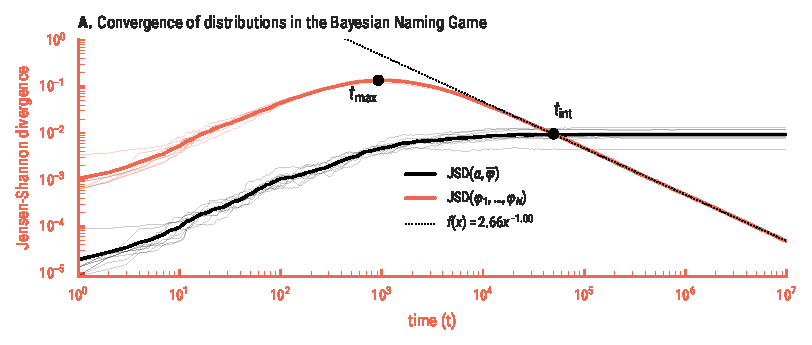
\includegraphics[trim=1.26cm 0 0 \figtopmargin]{BNG02-results}
	
	\caption{%
	The Dirichlet-categorical name converges to a stable, coherent language.
	\subfig{A} The distance between expected languages vanishes, but the aggregate language deviates from the bias. 
	\subfig{B} Coherence initially drops, but then increases to 1. The black line illustrates the \emph{reflection of the bias}.
	%--------
	\figdetails{\figid{bng02} %
	$K=40$, $N=20$, $\eta=\zeta=1$, $\gamma=\infty$, $\beta=40$}
	\label{fig:BNG02-results}}
\end{SCfigure}
%- - - - - - - -




However, the stable language is \emph{not} identical to the bias. 
Rather, the effect of the bias diminishes as can be seen from the reflectance (figure \ref{fig:BNG02-results}\textsc{b}, black).
The reflectance decreases, signalling a \emph{divergence} from the bias, until it stabilises below $R=1$.
The final reflectance is fairly consistent across runs and seems to be determined by the strength $\beta$ of the    (see below).
In summary, in every run of cultural evolution, in every lineage, the population develops a different, stable and shared language that reflects the innate biases, but diverges from it within certain bounds.



%- - - - - - - -
\begin{SCfigure}
	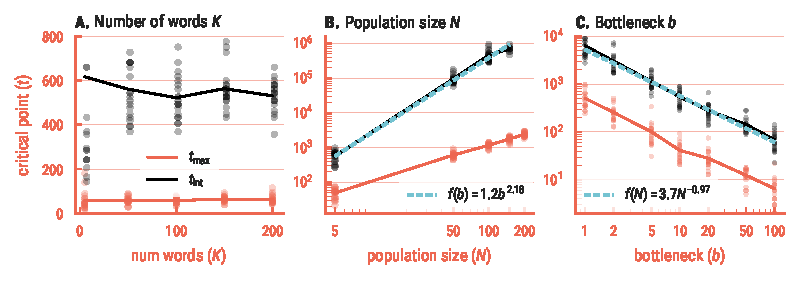
\includegraphics[trim=1.26cm 0 0 \figtopmargin]{BNG03-effects-params-on-convergence}
	\caption{Effects of the language, population and bottleneck size on convergence time, probed by the critical points $t_{\text{max}}$ and $t_{\text{int}}$. See main text for details.
		\figdetails{\figid{bng03}
		Parameters are fixed at $N=5$, $K=10$ and $b=10$, if they are not varied.
		$\eta=\zeta=1$, $\gamma=\infty$, $\beta=100$.}
		\label{fig:BNG03-effects-params-on-convergence}}
\end{SCfigure}
%- - - - - - - -




%——————————————————————————————————————————————————————————
\paragraph{scaling}

Figure \ref{fig:BNG02-results} highlights two ‘critical’ points $t_{\text{max}}$ and $t_{\text{int}}$, namely the maximum of $\textsc{jsd}(\vect\pi_1, \dots, \vect\pi_N)$ and the intersection of that with $\textsc{jsd}(\bar{\vect\pi}, \hat{\vect\alpha}_0)$ respectively.
These points seem to provide reliable indications of the convergence time and can thus be used to analyse how it is influenced by different parameters \parencite[cf.][]{Baronchelli2008,Baronchelli2017}.
Figure \ref{fig:BNG03-effects-params-on-convergence} shows the effects of the language size ($K$), the population size ($N$) and the bottleneck size ($b$) on the convergence time, measured by the location of $t_{\text{max}}$ and $t_{\text{int}}$.
The number of words does not seem to have a strong effect on the convergence time. 
This is somewhat surprising and it might be worth investigating further.
The population size does have a clear effect and seems to follow a power law $t_{\text{int}} \propto N^{2.18}$ (estimated using linear regression).
The minimal naming game exhibits similar power-law scaling, although with a different exponent of 1.5 (see \eqref{eq:ch3:scaling-naming-game}).
This means that convergence time increases quickly as the population grows.
But, as subfigure \textsc{c} shows, growing convergence times can be countered by increasing the bottleneck.
This, too, exhibits power-law behaviour $t_{\text{int}} \propto b^{-.97}$, which is suspiciously close to $t_{\text{int}} \propto b^{-1}$.
This is not surprising since larger bottlenecks allow for a more faithful transmission of the language, leading to faster convergence.
Finally it should be stressed that the numerical results are rather rough estimates, since the explored range is very limited.
Future work might extend the range to obtain more reliable numbers, or search for analytic results.
%%



%- - - - - - -
\begin{SCfigure}
	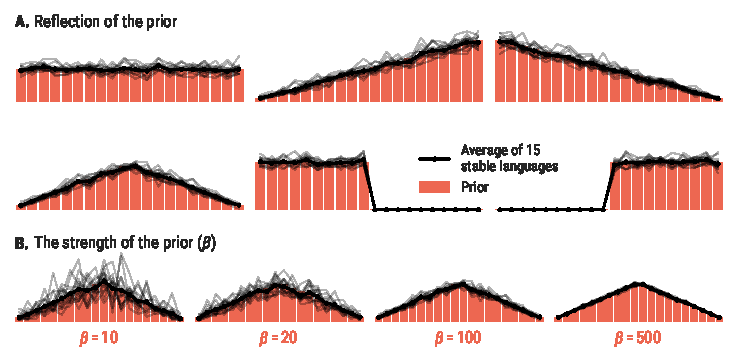
\includegraphics[trim=0.26cm 0 0 \figtopmargin]{BNG04-07-reflection-prior}
	
	\caption{\subfig{A} %
	Different runs of evolutionary history result in different stable languages (thin black lines) that all reflect the prior (orange) in the sense that cultural evolution reproduces the prior \emph{on average} over many runs. 
	This is illustrated with six differently shaped priors.
	\subfig{B} How well the languages reflect the prior is regulated by the strength of the prior ($\beta$).
	%----------
	\figdetails{\figid{bng04/07} 
	$K=20$, $N=10$, $b=10$, $\zeta=\eta=1$, $\gamma=\infty$, $\beta=100$}
	\label{fig:BNG04-07-reflection-prior}}
\end{SCfigure}
%- - - - - - -




%——————————————————————————————————————————————————————————
\paragraph{reflection of the bias}

What mechanism underlies the ‘reflection of the bias’ in the final language?
One possibility is that every converged language is a ‘draw’ from some distribution around the bias.
That would mean that cultural evolution reproduces innate biases, but only \emph{on average}.
To test this, the game was repeated 15 times with six differently shaped biases.
Indeed, each of the 15 lineages developed a distinct language, but the average of all lineages closely aligns with the innate bias (see figure \ref{fig:BNG04-07-reflection-prior}\textsc{a}).
The next question might be how much the emerging languages can deviate from the bias. 
This, it seems, is determined by the strength of the bias, $\beta$. 
Recall that the bias enters the model as the parameter of a Dirichlet distribution and $\vect\alpha_0$ can thus be factorised as $\vect\alpha = \beta\cdot\vect\mu$ where $\beta$ is an inverse variance for the corresponding Dirichlet. 
Higher values of $\beta$ result in smaller variance.
This translates directly to the distance the resulting languages can have from the bias, as illustrated by figure \ref{fig:BNG04-07-reflection-prior}\textsc{b}.
These results corroborate the idea that in this model, cultural evolution effectively samples a language from a distribution around the bias. 
Interestingly, the resulting pattern is a common one in linguistics: \emph{wide constrained variation} \parencite{Regier2015}.
Colour terms, to name one example, vary across languages, but within certain constraints \textcite{Regier2015}.






%——————————————————————————————————————————————————————————
%——————————————————————————————————————————————————————————
\section{Language and production strategies}
%——————————————————————————————————————————————————————————
%——————————————————————————————————————————————————————————




%——————————————————————————————————————————————————————————
\paragraph{language strategies}

Chapter \ref{ch:iterated-learning} discussed two strategies for selecting languages in iterated learning models: sampling a language or using the maximum of the posterior (\textsc{map}).
The same strategies can be introduced in Bayesian naming games, using a parameter $\eta$ to interpolate between them.
In the Dirichlet-categorical model, the exponentiated distribution even has a simple analytical form (see \eqref{eq:app-bng:exponentiated-dirichlet}):
%-
\begin{align}
	p_\LA(\vlang \mid \vect x, \vect\alpha) 
		&\propto \bigl[p\bigl(\vlang \mid \vect x, \vect\alpha\bigr)\bigr]^\eta
		\\
		&= \text{Dirichlet}(\vlang \mid \eta\cdot (\vect\alpha - \vect1) + \vect1).
\end{align}
%-
Exponentiation shifts the distribution towards its mode, the point with highest probability, and moreover shrinks the variance, as illustrated in  figure \ref{fig:dirichlet-eta}.
We assume that agents only use the exponentiated posterior during \emph{production}, and use the normal (un-exponentiated) posterior as the prior in the next round. 
In other words, a hearer updates its beliefs to $\vect\alpha_{t+1} := \vect\alpha_t + \vect c_t$, and \emph{not} to $\eta (\vect\alpha_t - \vect 1) + \vect 1 + \vect c_t$.
This means that agents will use the (internal) language they are most confident about, but remember how uncertain they were about other languages.
After all, if an agent were to use the exponentiated posterior as the prior in the next round, it would effectively assume that the language it last encountered will from now on be used by all other agents.
For that reason $\eta$ really determines a production strategy, and not a \emph{learning strategy} (the name commonly used in \textsc{il}).
I have called it the \emph{language} strategy to distinguish it from the actual production strategy (see below, and also figure \ref{fig:ch4-bng-terminology}).




%- - - - - - - 
\begin{SCfigure}
	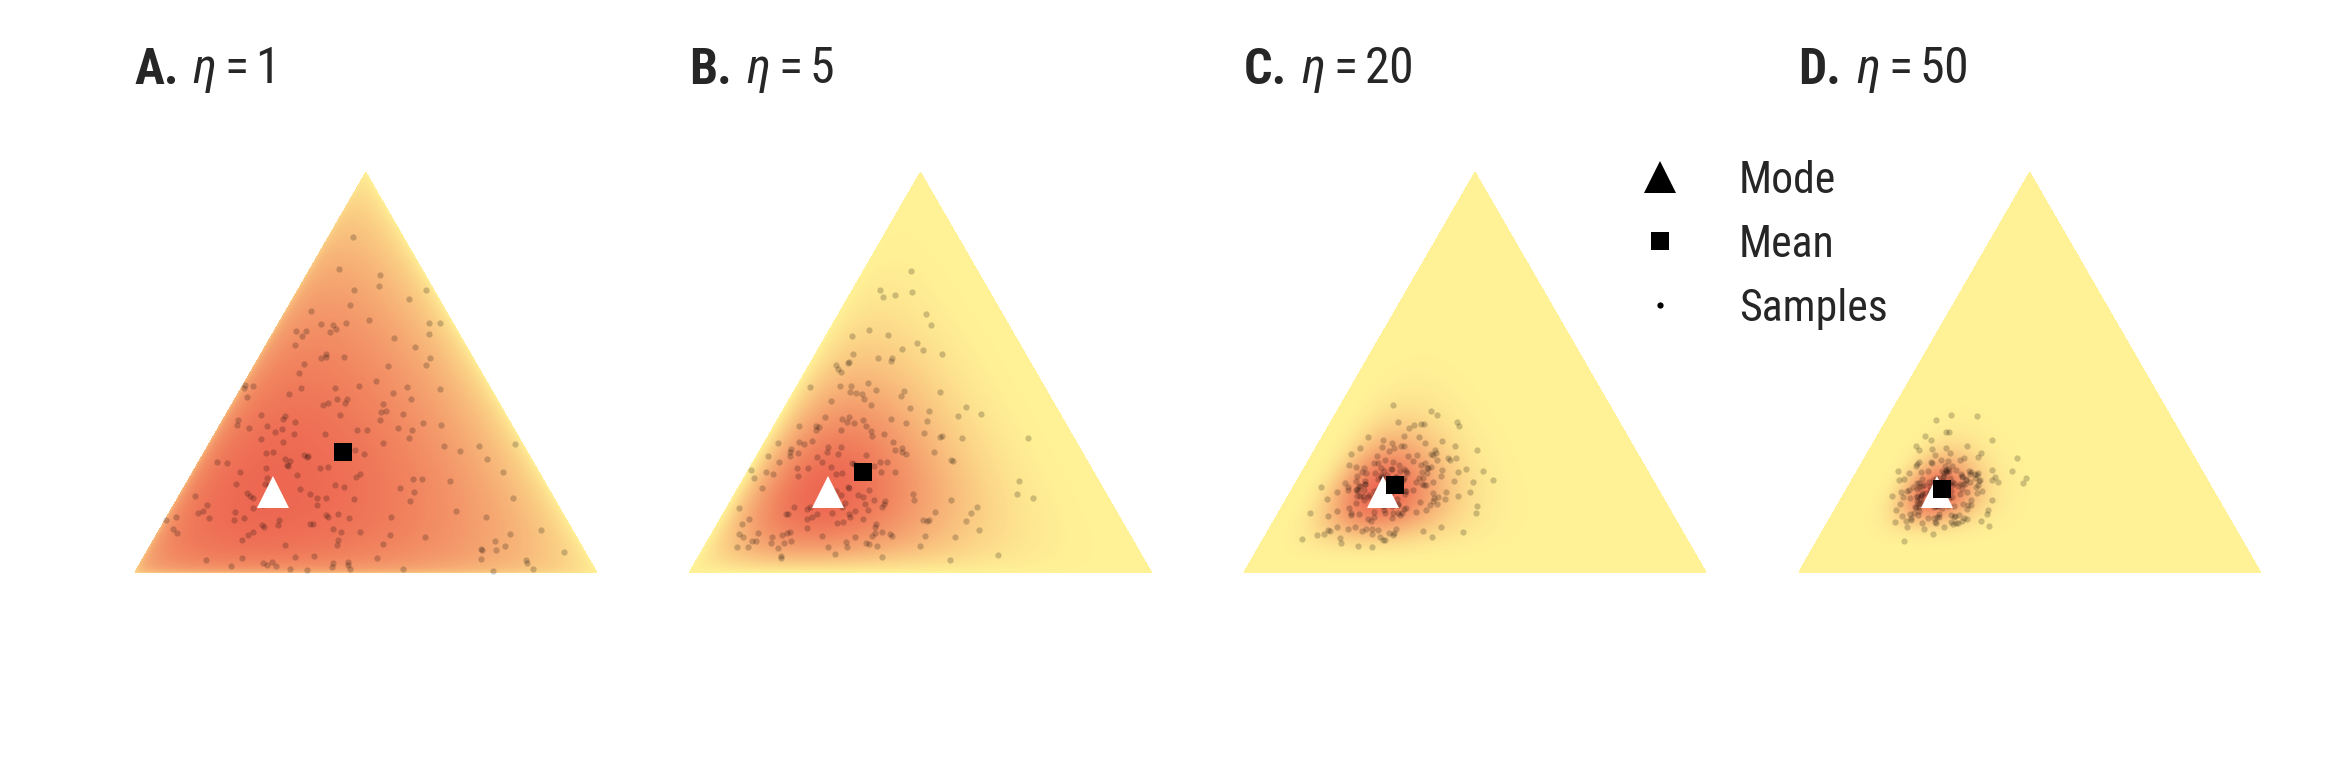
\includegraphics[trim=0.94cm 0 0 \figtopmargin]{FIG02-dirichlet-eta}
	
	\caption{Exaggerating (or exponentiating) a Dirichlet distribution shrinks the variance and as $\eta$ grows, the mean approaches the mode. 
	%----------
	\figdetails{\figid{fig02}}
	\label{fig:dirichlet-eta}}
\end{SCfigure}
%- - - - - - - 




%——————————————————————————————————————————————————————————
\paragraph{production strategies}

In a similar fashion, different strategies for picking \emph{words} can be defined by sampling from
%-
\begin{equation}
	p_\PA(x \mid \vlang, \vect\alpha) 
		\propto \bigl[\; p(x \mid \vlang, \vect\alpha) \;\bigr]^\zeta.
\end{equation}
%-
One reason for introducing the \textsc{map}-strategy for selecting utterances (i.e., $\zeta = \infty$) is that it mirrors the production strategy used in naming games.
There, agents typically produce the word with the highest score.
But if we assume, following \textcite{Griffiths2007a}, that agents are Bayesian and have accurate knowledge of the production strategy, they should infer a different posterior distribution: $p(\vlang \mid x) \propto p_\PA(x \mid \vlang) \cdot p(\vlang)$.
This distribution is no longer a Dirichlet distribution (see appendix \ref{app:bng}) and a result, posterior inference cannot take the form of updating $\vect\alpha$.
This significantly complicates the game and partly for that reason we assume that agents update their posterior \emph{without} taking into account $\zeta$.
\emph{For $\zeta > 1$ agents are therefore not (perfect) Bayesian reasoners.}
This, I would argue, is not too problematic, since the parameter $\zeta$ is primarily introduced to reproduce the naming game, which itself does not use Bayesian agents. 
Moreover, technical considerations suggest that Bayesian agents that \emph{do} take into account $\zeta$ would after a single observation deem all  languages to be absurd, if they do not assign the highest probability to the observed word. That also seems unrealistic.\footnote{%:
	%>>>
	But then again, this probably happens because agents do not take into account that the language comes from multiple sources \parencite[cf][]{Ferdinand2009,Smith2009} and is discussed later.
	%<<<
	}
%%



In short, a round in the Dirichlet-categorical naming, with language and production strategies parametrised by $\eta$ and $\zeta$, takes the following form
%-
\begin{align}
	&\textsc{speaker} 
	\quad
	\begin{cases} 
		\;\vlang_t \mid \vect\alpha_{t-1}
			&\sim \text{Dirichlet}\bigl(\;\eta(\vect\alpha_{t-1} - 1) + 1\;\bigr)
			\\[.5em]
		\;x_i \mid \vlang_t
			&\sim \text{Categorical}\bigl( \vlang^\zeta / \vectsum{\vlang^\zeta} \bigr), \quad i = 1, \dots, b.	
	\end{cases}
	\\[.5em]
	%- - - - - - - -
	&\textsc{hearer} 
	\qquad \;\;
	\vect\alpha_{t+1} 
			:= \vect\alpha_t + \vect c_t
\end{align}
%-
where $\vectsum{\vect \vlang^\zeta} := \lang_1^\zeta + \dots \lang_K^\zeta$ denotes the sum of the entries of a vector.
%%





In conclusion, Bayesian naming games can use different language and production strategies by importing parameters $\eta$ and $\zeta$ from iterated learning and naming games respectively.
We will evaluate all these strategies empirically and, in some cases, analytically.
But it is better to do that later, in tandem with a new population structure that connects the Bayesian naming game to Bayesian models of iterated learning.







%——————————————————————————————————————————————————————————
%——————————————————————————————————————————————————————————
\section{Bayesian language games}
%——————————————————————————————————————————————————————————
%——————————————————————————————————————————————————————————


The Bayesian naming game was directly inspired by Bayesian models of iterated learning.
The strategies, we have just seen, can also be connected to strategies used in the naming game.
We now take the analogies one step further and explicitly connect the two paradigms.
I reserve the name \emph{Bayesian naming game} for the game studied above, and refer to the extension that we will define here as the \emph{Bayesian language game}, since it includes iterated learning-type models.
To connect iterated learning to the Bayesian naming game, the population model has to be changed.
I propose to add two ingredients: random walks and a life expectancy.
The model will do a random walk through a population of fixed size. 
If agents ‘die’ after every interaction, the random walk becomes a transmission chain used in iterated learning.
If the agents live forever, the random walk resembles homogeneous mixing from the naming game.
Random walks might not be a very realistic model of linguistic interaction (although similar to homogeneous mixing), but formulating the most realistic model is not our main motivation either. 
Rather, connecting the two paradigms aims to highlight what they have in common and where they diverge.
%%




%- - - - - - - 
\begin{SCfigure}\footnotesize
	%\documentclass{../src/bcthesispart}
%\begin{document}
\begin{tikzpicture}[xscale=1.2, yscale=.75]
	  \tikzset{agent/.style={circle,fill=main,draw,minimum size=.3cm,inner sep=0pt},
            }
		\tikzset{interaction/.style={shorten >=0.15cm,shorten <=.15cm,thick}}

	% Iterated Learning
	\begin{scope}
	 	\foreach \y in {2,1,0,-1} {
	 		\node[agent] at (0, \y) { };
	 	}
	 	
	 	\draw [interaction,->] (0, 2) -- (0, 1);
	 	\draw [interaction,->] (0, 1) -- (0, 0);
	 	\draw [interaction,->] (0, 0) -- (0, -1);
	 	\draw [interaction,->] (0, -1) -- (0, -2);
	 	
	 	\node[align=center,below] at (0,-3) {\sffamily \textsc{transmission chain}\\\sffamily Iterated learning};
	\end{scope}

	% Naming Game
	\begin{scope}[xshift=1.5cm]
	 	\foreach \x in {0,...,3} {
	 		\node[agent] at (\x, 0) {}; 
	 	}
	 	\foreach \y in {-1,1 } {
	 		\foreach \x in {.5,1.5,2.5} {\node[agent] at (\x, \y) { }; }
	 	}
		\foreach \y in {-2,2 } {
	 		\foreach \x in {1,2} {\node[agent] at (\x, \y) { }; }
	 	}
	 	
	 	\draw [interaction,->] (2, 2) -- (2.5, 1);
	 	\draw [interaction,->] (1, 2) -- (.5, -1);
	 	\draw [interaction,->] (1, 0) -- (2.5, -1);
	 	\draw [interaction,->] (1.5, -1) -- (3, 0);
	 	\draw [interaction,->] (2, -2) -- (1, -2);
	 	\draw [interaction,->] (1, 2) -- (.5, 1);
	 	\draw [interaction,->] (1.5, 1) -- (2, 2);
	 	\draw [interaction,->] (2, 0) -- (1.5, -1);
	 	\draw [interaction,->] (0, 0) -- (1.5, 1);
	 	\draw [interaction,->] (1, -2) -- (1, 0);
	 	
	 	\node[align=center,below] at (1.5,-3) {\sffamily \textsc{homogeneous mixing}\\\sffamily Naming Game};
	\end{scope}
	
	% Bayesian Naming Game
	\begin{scope}[xshift=6cm]
	 	\foreach \x in {0,...,3} {
	 		\node[agent] at (\x, 0) {}; 
	 	}
	 	\foreach \y in {-1,1 } {
	 		\foreach \x in {.5,1.5,2.5} {\node[agent] at (\x, \y) { }; }
	 	}
		\foreach \y in {-2,2 } {
	 		\foreach \x in {1,2} {\node[agent] at (\x, \y) { }; }
	 	}
	 		 
		\draw [interaction,->] (2, 2) -- (2, 0);
	 	\draw [interaction,->] (2, 0) -- (3, 0);
	 	\draw [interaction,->] (3, 0) -- (2.5, -1);
	 	\draw [interaction,->] (2.5, -1) -- (1, -2);
	 	\draw [interaction,->] (1, -2) -- (1, 0);
	 	\draw [interaction,->] (1, 0) -- (0.5, -1);
	 	\draw [interaction,->] (0.5, -1) -- (0,0);
		\draw [interaction,->] (0,0) -- (1.5, 1);
		\draw [interaction,->] (1.5, 1) -- (1,2);	
		
	 	\node[align=center,below] at (1.5,-3) {\sffamily \textsc{random walk}\\\sffamily Bayesian Naming Game};
	\end{scope}
\end{tikzpicture}

%\end{document}

	
	\caption{%
	The proposed transmission model, a random walk through the population, combines the transmission chains used in iterated learning with the homogeneous mixing from the naming game.
	\label{fig:ch4:population-structures}}
\end{SCfigure}
%- - - - - - - 




%——————————————————————————————————————————————————————————
\paragraph{Ingredient 1: random walks}

Transmission chains and homogeneous mixing are naturally combined into a random walk (see figure 
\ref{fig:ch4:population-structures}).
Starting with a random first agent, in every round only one new agent is selected. 
The previous hearer becomes the next speaker.
In that way a path through the population is formed that, when unraveled, mirrors a transmission chain.
This trick is also used by \textcite{Whalen2017} in the context of arbitrary graphs.
Note that this walk does not impose any restrictions on which agents can interact.
Over time all agents are visited equally often and with equal probability.\footnote{%
	%>>>
	More precisely, the random walk is a Markov chain over the population with uniform stationary distribution.
	%<<<
	}
The underlying social network is fully connected and in that sense there is homogeneous mixing. 
Note that using a random walk in the \emph{minimal} naming game would be rather pointless: only the first agent will invent a word, which then spreads the population.
This is caused by the extreme form of lateral inhibition, and the Bayesian language game seems unaffected by this.\footnote{%
	%>>>
	I have not been able to isolate systematic differences between homogenous mixing and random walks in the Bayesian language game, although future work could investigate this more systematically
	%<<<
	}
%%





%——————————————————————————————————————————————————————————
\paragraph{Ingredient 2: vary the life expectancy}

Although a random walk forms a chain, it is not a typical \emph{transmission chain} since agents can join in several times.
For iterated learning, this issue is particularly pressing — you would not want the great-grandmothers to reappear as the children of their great-granddaughters.
Fortunately, this is easily remedied by the second ingredient: death.
If speakers were to die after every encounter, and if their places were taken by newborns, the random walk \emph{does} reduce to a transmission chain.
Conversely, if agents live forever one retrieves the naming game.
And for intermediate life expectancies, one gets a gradual turnover of the population with both horizontal interactions (between agents that have lived for a while) and vertical interactions (between newborns and older agents) — a bit like the real world.



Birth-death processes are fairly common in the language evolution literature.
To cite just two examples, \textcite{DeBoer1999} and \textcite{Smith2002} model population turnover by removing one random agent in every round, and replacing it with a new agent.
The problem with this approach is that it implies a rather unrealistic model of life-expectancy.
To see why, one has to look at the so called \emph{hazard rate}: probability that an agent will die in a given round, given that it is not dead yet \parencite{Rodriguez2007}.
In the mentioned studies, this quantity is constant: $\nicefrac{1}{N}$.
Constant hazard rates do arise naturally, for example in radioactive decay, but not in human mortality rates.
Those are much higher amongst elderly (and infants) and therefore not constant.
For that reason, demographers have adopted different models often building on either the \emph{Weibull} or \emph{Gompertz} distribution \parencite{Juckett1993}.


%- - - - - - - 
\begin{SCfigure}\footnotesize
	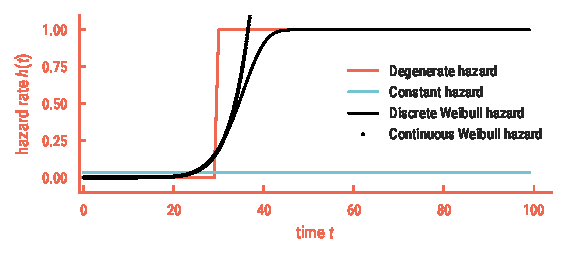
\includegraphics[trim=1.31cm 0 0 \figtopmargin]{FIG04-hazard-functions}

	\caption{%
	Different hazard functions.
	The more realistic (continuous/discrete) Weibull hazard is better approximated by a degenerate than a constant hazard function.
	\label{fig:ch4:hazards}}
\end{SCfigure}
%- - - - - - - 



In appendix \ref{app:weibull} I have outlined a \emph{discrete Weibull} model of life expectancy.
It has one parameter $\gamma$, which is the average life-expectancy.
Since mathematical analyses might benefit from an even simpler model, I alternatively propose to use a \emph{degenerate hazard} function that assigns all agents an identical, fixed life-span.
This seems a better approximation of the Weibull than a model with constant hazard-rate (see figure \ref{fig:ch4:hazards}).
In the simulations below, I have indeed used a degenerate model with a fixed life-expectancy of $\gamma$, i.e. every agent dies after $\gamma$ interactions as a speaker.\footnote{%
	%<<<
	Here too, I have to leave it to future work to \emph{systematically} assess the impact of the different models of population turnover.
	%<<<
	}






%——————————————————————————————————————————————————————————
%——————————————————————————————————————————————————————————
\section{Characterising Bayesian language games}
%——————————————————————————————————————————————————————————
%——————————————————————————————————————————————————————————



The \emph{Bayesian language game} is simply the Bayesian naming game extended with the random walk and population turnover outlined above.
It can reproduce various different models, depending on three parameters:
%...
\begin{itemize}
	\item \textbf{Language strategy $\eta$}. Determines to what extend the agents favour more likely languages. $\eta=1$ yiels samplers, $\eta=\infty$ maximisers.
	\item \textbf{Production strategy $\zeta$.} Regulates the tendency to produce more likely productions; $\zeta=1$ for samplers and $\zeta=\infty$ for maximisers.
	\item \textbf{Life expectancy $\gamma$.} The average life expectancy of an agent in terms of the number of rounds it can play as a speaker. For $\gamma=1$ for iterated learning; $\gamma=\infty$ for a naming game.
\end{itemize}
%...
Of course, the population size, number of words and bottleneck size are also of interest, but $\eta, \zeta$ and $\gamma$ most directly determine the type of game.
The next question is simple: how?
What kind of behaviour can we expect for different parameter settings?
To find out, an experiment was set up to explore a larger part of the parameter space $(\eta, \zeta, \gamma)$ in a systematic fashion.
The parameters appear to interpolate relatively smoothly between the extreme cases where $\eta,\zeta$ and $\gamma$ are either $1$ or $\infty$.
The extreme cases are, I believe, most clearly illustrated by the outcomes of single runs.
The main text discusses those, and I refer to appendix \ref{app:bng-params} for a more systematic exploration of the parameter space confirming the findings discussed here.




The central figure is \ref{fig:FIG08-bng-overview}.
It shows one run of the Dirichlet-categorical language game for four different life expectancies: $\gamma=1$ (iterated learning), $\gamma=\infty$ (naming game) and the intermediate $\gamma=10$ and $\gamma=100$.
For every $\gamma$ the four ‘extreme’ language-production strategies $(\eta,\zeta)$ are shown: sample-sample, sample-\textsc{map}, \textsc{map}--sample and \textsc{map--map}.
Note that the blue bars show the external language, not the prior.
All runs use the same prior: the by now familiar ‘pyramid’.
I first discuss the effect of population turnover ($\gamma$) and then turn to the different strategies.




%- - - - - - - - 
\begin{SCfigure}
	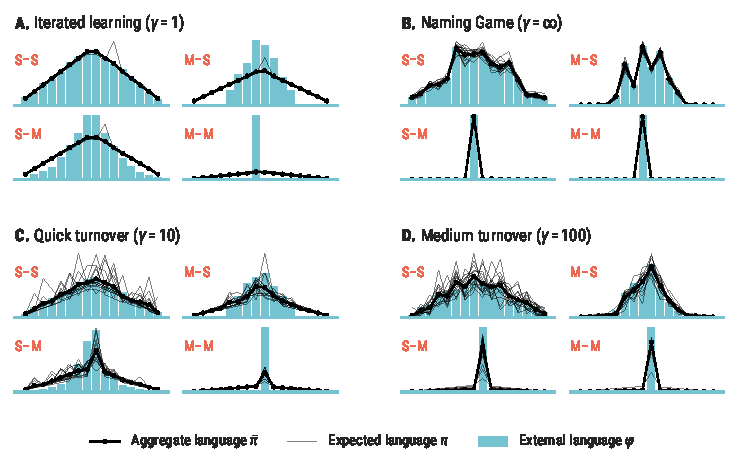
\includegraphics[trim=0.2cm 0 0 \figtopmargin]{FIG08-BNG-overview}
	
	\caption{%
	Typical outcomes of the Dirichlet-Categorical language game for the extreme strategies 
	(sample--sample, \textsc{map}--sample, sample--\textsc{map}, \textsc{map--map}) in populations with 
	immediate turnover (\textsc{a}, iterated learning, $\gamma=1$), 
	no turnover (\textsc{b}, naming game, $\gamma=\infty$) 
	and two intermediate turnovers (\textsc{c} and \textsc{d}).
	See the main text for a discussion.
	\figdetails{\figid{fig08} 
	$K = 16$, $N = 15$, $b = 1$, $T=10 000$}
	\label{fig:FIG08-bng-overview}}
\end{SCfigure}
%- - - - - - - - 




\paragraph{Varying life expectancy: between \textsc{il} and \textsc{ng}’s}

The results for iterated learning (subfigure \textsc{a}), are easily misinterpreted.
At every point, only one agent has some past experience: the current speaker.
That speaker corresponds to the thin line deviating from the aggregate language.
The expected language of all other agents is exactly their bias.
Through the lens of the Bayesian language game, we see an almost perfectly homogeneous population, which explains why the aggregate language $\bar{\vect\pi}$ is the same for all strategies.
This also means that the coherence is near-maximal, but this could be seen as an artefact.
After all, considering the external language reveals an important discrepancy for non-sampling strategies.
The internal language of agents, as seen from the aggregate language, is in strong disagreement with the external language (orange).
That means that no agent, not even the speaker, has a faithful internal representation of the language actually used.
With more experience the discrepancy disappears: in naming game (subfigure \textsc{b}) the external and internal languages are in fair agreement.
More experience can also result from larger bottlenecks, which would result in  only the speaker having a better representation of the language.




Another interesting observation is suggested by the two mixed strategies, \textsc{map}--sample and sample--\textsc{map}.
Both exaggerate the bias, but in different ways.
Maximising only the language appears to \emph{prune} low-probability languages, whereas maximising only productions seems to \emph{exponentiate} the language.
This would explain the shape of the limiting language under a \textsc{map}--sample strategy in the naming game.
That appears to consistently deviate from an exponentiated distribution and indeed more closely resembles a pruned distribution.
Needless to say, more work is needed to confirm this ‘pruning-vs-exponentiating’ hypothesis.
The most striking difference between the Bayesian iterated learning model and the naming game is the ‘predictability’ of cultural effects with the former.
Even maximising strategies appear to result in languages that are determined by the bias, and some simple operation (possibly pruning or exponentiating).
They are seemingly uninfluenced by the contingencies of the cultural process, in sharp contrast to the Bayesian naming game.
This suggests that even maximising strategies in Bayesian iterated learning result exhibit fairly “uninteresting” \parencite[cf.][]{Dediu2009} behaviour.





The Bayesian naming game arguably exhibits more “interesting” behaviour, since the resulting languages are clearly shaped by a the contingencies of a rough, stochastic process of cultural evolution.
The intermediate life expectancies seem to interpolate between \textsc{il} and \textsc{ng} behaviour.
The longer the agents live, the — yes — ‘stronger and stabler’ the cultural effects become, and the more languages can move away from the biases.
For intermediate languages, variability can be large since new agents can always be introduced.
An interesting question if the Bayesian language game can also reproduce gradual language change while maintaining a fair stability.
Preliminary experiments suggest this is the case (see figure \ref{fig:FIG11-BNG-language-change}, although they also suggest that the effect is brittle in the sense that for example increasing $\gamma$ quickly seems to result in behaviour more similar to $\gamma=\infty$.




%- - - - - - - - 
\begin{SCfigure}
	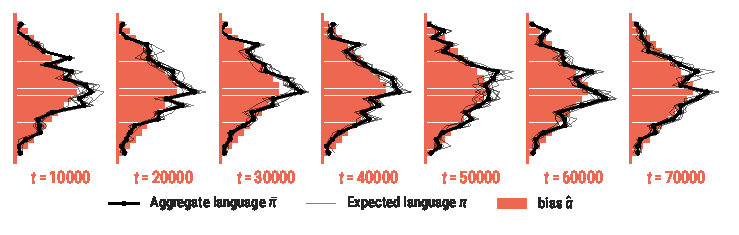
\includegraphics[trim=0.2cm 0 0 \figtopmargin]{FIG11-BNG-language-change}
	
	\caption{%
	Gradual language change in the Bayesian language game for a particular choice of parameters.
	The effect seems brittle: slightly different parameter settings can give the kind of behaviour shown when $\gamma=\infty$.
	%----------
	\figdetails{\figid{fig11} 
	$K = 20$, $N = 10$, $b = 2$, $\beta = 40$, $\gamma=700$, $\eta=2$, $\zeta=1$, deterministic hazard.}
	\label{fig:FIG11-BNG-language-change}}
\end{SCfigure}
%- - - - - - - - 




%——————————————————————————————————————————————————————————
\paragraph{Extreme strategies for the Bayesian naming game}

The Bayesian \emph{naming} game implements a kind of lateral inhibition in the form of Bayesian updating.
So do other strategies correspond to the different alignment strategies in the naming game?
I discuss all strategies below, also $\gamma < \infty$/
%...
\begin{itemize}
\item \textbf{Sample--sample (\textsc{s--s}, $\eta=\zeta=\infty$).}
	This is the ‘default’ strategy in the Bayesian naming game and corresponds to the sampler-strategy in iterated learning.
	This strategy exhibits lateral inhibition, in the sense that the ‘score’ of an observed word increases, while the score of other words decrease.
	By \emph{score} the probability of the word under the expected language $s_t(x) := p(x \mid \vect\alpha_t)$ is meant. After observing $x_t$ it can be shown (see \eqref{eq:app-bng:update-sampler}) to change to
	%-
	\begin{align}
		s_{t+1}(y) =
			\frac{\vectsum{\vect\alpha_t}}%
				{\vectsum{\vect\alpha_t} + 1} 
			\cdot s_t(y)
			+ \frac{\ind{y=x}}%
				{\vectsum{\vect\alpha_t} + 1},
	\end{align}
	%-
	where $\ind{\text{ condition }}$ is the indicator function evaluating to 1 if the condition holds, and 0 otherwise.
	The update differs from the basic lateral inhibition strategies \parencite[e.g.][]{Wellens2012}.
	First, the inhibition works by scaling rather than subtraction of a fixed parameter $\delta_{\text{inh}}$. 
	Second, the effect of the updates decreases with time since $\vectsum{\vect\alpha_t}$ increases over time.
	Note that this proves that the expected language of one particular agent will converge, since the updates vanish.
	The simulations earlier this chapter suggest that all agents moreover converge to the same language, which reflects the bias.
	This is also what we see in figure \ref{fig:FIG08-bng-overview}\textsc{b} (\textsc{s--s}).
	%...
%	\begin{itemize}
%		\item \emph{Alignment:} variant of lateral inhibition
%		\item \emph{Language:} reflects the bias
%	\end{itemize}
	%...

	

%% MAP - Sample
\item \textbf{\textsc{map}--sample (\textsc{m--s}, $\eta=\infty, \zeta=1$).}
	This strategy is used by maximisers in iterated learning. 
	The lateral inhibition mechanism takes a very similar form as in the sample-sample strategy.
	In particular, the updates eventually also vanish, proving ‘individual’ convergence.
	Simulations suggest that coherence always emerges and the stable language appears to reflect an amplified or exaggerated version the bias.
	The exaggeration is apparent from figure \ref{fig:FIG08-bng-overview}\textsc{b} (\textsc{m--s}), where the resulting language is more peaked than the prior.
	The prior is not shown, but is the ‘pyramid’ also visible in subfigure \textsc{a} (\textsc{s--s}). 
	%...
%	\begin{itemize}
%		\item \emph{Alignment:} variant of lateral inhibition
%		\item \emph{language:} reflects an amplified bias
%	\end{itemize}
	%...


% Sample - MAP
\item \textbf{Sample--\textsc{map} (\textsc{s--m}, $\eta=\infty, \zeta=1$).}
	This strategy is hardest to analyse, since the scores $p(x \mid \vect\alpha)$ do not seem to have a simple expression (see appendix \ref{app:bng} for details).
	However, when bias is flat the strategy reduces to the case analysed by \textcite{DeVylder2006}, which implies convergence to a single-word language.
	Indeed figure \ref{fig:FIG08-bng-overview}\textsc{b} (\textsc{s--m}) confirms that idea.
	%...
%	\begin{itemize}
%		\item\emph{Alignment:} unknown
%		\item\emph{language:} single-word
%	\end{itemize}
	%...
	 
% MAP - MAP
\item  \textbf{\textsc{map}--\textsc{map} (\textsc{m--m}, $\eta=\zeta=\infty$).}
	The \textsc{map--map} strategy corresponds to the frequency strategy from chapter \ref{ch:naming-games}.
	An agent with this strategy uses the language with highest probability, the mode, and then utters the largest component from the mode. 
	This amounts to producing $x_t = \argmax_k \vect\alpha_k$, the word with the highest counts, including pseudo-counts.
	The only words these agents will every use are the maxima of the bias.
	Consistent with chapter \ref{ch:naming-games}, we find convergence to a single-word language in \ref{fig:FIG08-bng-overview}\textsc{b} (\textsc{m--m}). 
%	\begin{itemize}
%		\item\emph{Alignment:} frequency strategy
%		\item\emph{language:} single-word
%	\end{itemize}

\end{itemize}
%...



\section{Conclusions}


This chapter proposed a Bayesian naming game based on a Dirichlet-categorical model.
In the standard version of the game ($\eta=\zeta=1$) the population reaches coherence in a typical three-stage process, metaphorically called ‘infancy’, ‘puberty’ and ‘adulthood’.
The resulting language reflects the bias, but is clearly shaped by the contingencies of cultural evolution.
The model thus gives rise to lineage-specific, stable languages.
In sum, it answer many of the desiderata formulated in chapter \ref{ch:iterated-learning}. 
Concretely, it explicitly represents biases \ref{desideratum:biases};
incorporates strategies from both the iterated learning and naming game literature \ref{desideratum:strategies};
seems susceptible to mathematical analysis \ref{desideratum:analysable}, as further discussed in chapter \ref{ch:conclusions};
exhibits nontrivial cultural effects \ref{desideratum:cultural-effects}; 
and results in a stable language (\ref{desideratum:stable}).



The Bayesian \emph{naming} game was extended to the Bayesian \emph{language} game by introducing language- and production strategies ($\eta$ and $\zeta$) and a population model consisting of (1) a random walk and (2) a life expectancy $\gamma$ for every agent.
For $\gamma=1$ this produced an iterated-learning model, for $\gamma=\infty$ in a naming game.
A characterisation of the parameter space suggested several conclusions.
First, that agents in an iterated learning model never faithfully represent the language actually used.
And second, that the effect of maximising languages or productions are different and correspond to something like pruning or exponentiating the bias respectively.
This in turn indicates that for those strategies are also relatively ‘uninteresting’ in iterated learning models, in the sense that that the outcome seems to be predictably determined by the bias.
This is not the case for the Bayesian naming game, where the cultural process leaves a non-trivial on the language.
That does not mean that the process is completely unpredictable, since the resulting language appears to be a draw from some distribution around the prior, allowing for only limited variability.




An interesting further question concerns ‘stable’ language change. 
Initial results suggest this can occur, but is somewhat brittle and does therefore not fulfil the desideratum of robustness (\ref{desideratum:robust}).
In general, the characterisation however does suggest a fair robustness.
All small values of $\gamma$ result in behaviour very similar to $\gamma=0$ (iterated learning), and all large values are similar to $\gamma=\infty$.
The same goes for the strategies: there seems to be a relatively smooth transition between the extreme cases.
That means that understanding the extreme cases gives a fair sketch of the kind of behaviour that can be expected.
In short, those are that sampling strategies result in (external) languages reflecting the biases, either perfectly (iterated learning) or imperfectly, when mediated by culture (naming game); 
mixed strategies exaggerate the biases, but differently when languages or productions are maximised (and again perfectly or imperfectly);
and pure maximising strategies result in degenerate distributions.
The longer the life span, the closer the external and internal languages align and the greater the language stability.




Of all the desiderata formulated in chapter \ref{ch:iterated-learning}, only one remains.
This is not to say that the models presented perfectly addressed all points, merely that they did so sufficiently for the purposes of this thesis — I discuss it’s shortcomings in the final chapter.
In the second part, I address the remaining desideratum: empirical testability.
Let me end this chapter with some remarks on related work.






\paragraph{related work}

The Bayesian iterated learning model is closely related to various models proposed in the literature.
In the naming game literature, \textcite{DeVylder2006} is the closest analogue I have been able to find.
The Dirichlet-categorical naming game nearly has their model as a special case, with a flat prior and a \textsc{map} language-strategy ($\eta=\infty$).
The queue-agents can be roughly approximated by a fixed life-expectancy corresponding the length of the queue, but the analogy is not perfect.
An interesting question is whether their results can be extended to the continuous case here.
Even more closely related is the model by \textcite{Reali2010}.
In fact, it is the exact same Dirichlet-categorical model, but only studied in the iterated learning context.\footnote{%
	%>>>
	I unfortunately only became aware of this while writing up the results and time does not allow me to include an in-depth discussion.
	%<<<
	}
Interestingly, they show that the model is in that case equivalent to the Wright-Fisher model of genetic drift.
Needless to say, this is an area ripe for future research.
The first sketches of a ‘Bayesian’ naming game can also be discerned in \textcite{Kirby2015}, who consider a population of two Bayesian agents interacting without population turnover.
\textcite{Ferdinand2009} similarly represent languages (hypotheses) as categorical distributions, but use a different prior.
A prior ‘extending’ the Dirichlet prior used here, the so called Dirichlet Process, has figured in \textcite{Burkett2010,Kirby2015}.
However, all these studies had different goals and none of them explicitly explored the parallels with naming games, hence I do not further discuss them here.


\showbibliography


\end{document}


%todo: bayesian cogn modelling
An arguably more principled mechanism uses Bayesian updating, which connects directly to work on Bayesian models of cognition \parencite[e.g.][]{Griffiths2010,Goodman2016}: 
